%%%%%%%%%%%%%%%%%%%%%%%%%%%%%%%%%%%%%%%%%%%%%%%%%%%%%%%%
\documentclass[12pt,a4paper]{article}% 文档格式
\usepackage{ctex,hyperref}% 输出汉字
\usepackage{times}% 英文使用Times New Roman
\usepackage[T1]{fontenc} % 保证英文字体加粗有效
%%%%%%%%%%%%%%%%%%%%%%%%%%%%%%%%%%%%%%%%%%%%%%%%%%%%%%%%
\title{\fontsize{18pt}{27pt}\selectfont% 小四字号,1.5倍行距
	{\heiti% 黑体 
		课程论文综述\LaTeX 模板}}% 题目
%%%%%%%%%%%%%%%%%%%%%%%%%%%%%%%%%%%%%%%%%%%%%%%%%%%%%%%%
\author{\fontsize{12pt}{18pt}\selectfont% 小四字号,1.5倍行距
	{\fangsong% 仿宋
		王小明}\thanks{标题栏脚注}\\% 标题栏脚注
	\fontsize{10.5pt}{15.75pt}\selectfont% 五号字号,1.5倍行距
	{\fangsong% 仿宋
		xxx大学~~~xxx学院}}% 作者单位,“~”表示空格
%%%%%%%%%%%%%%%%%%%%%%%%%%%%%%%%%%%%%%%%%%%%%%%%%%%%%%%%
\date{}% 日期(这里避免生成日期)
%%%%%%%%%%%%%%%%%%%%%%%%%%%%%%%%%%%%%%%%%%%%%%%%%%%%%%%%
\usepackage{amsmath,amsfonts,amssymb}% 为公式输入创造条件的宏包
%%%%%%%%%%%%%%%%%%%%%%%%%%%%%%%%%%%%%%%%%%%%%%%%%%%%%%%%
\usepackage{graphicx}% 图片插入宏包
\usepackage{subfigure}% 并排子图
\usepackage{float}% 浮动环境,用于调整图片位置
\usepackage[export]{adjustbox}% 防止过宽的图片
%%%%%%%%%%%%%%%%%%%%%%%%%%%%%%%%%%%%%%%%%%%%%%%%%%%%%%%%
\usepackage{bibentry}
\usepackage{natbib}% 以上2个为参考文献宏包
\usepackage{gbt7714}% 解决中文人名问题,引用变成右上角
%%%%%%%%%%%%%%%%%%%%%%%%%%%%%%%%%%%%%%%%%%%%%%%%%%%%%%%%
\usepackage{abstract}% 两栏文档,一栏摘要及关键字宏包
\renewcommand{\abstracttextfont}{\fangsong}% 摘要内容字体为仿宋
\renewcommand{\abstractname}{\textbf{摘\quad 要}}% 更改摘要二字的样式
%%%%%%%%%%%%%%%%%%%%%%%%%%%%%%%%%%%%%%%%%%%%%%%%%%%%%%%%
\usepackage{xcolor}% 字体颜色宏包
\newcommand{\red}[1]{\textcolor[rgb]{1.00,0.00,0.00}{#1}}
\newcommand{\blue}[1]{\textcolor[rgb]{0.00,0.00,1.00}{#1}}
\newcommand{\green}[1]{\textcolor[rgb]{0.00,1.00,0.00}{#1}}
\newcommand{\darkblue}[1]
{\textcolor[rgb]{0.00,0.00,0.50}{#1}}
\newcommand{\darkgreen}[1]
{\textcolor[rgb]{0.00,0.37,0.00}{#1}}
\newcommand{\darkred}[1]{\textcolor[rgb]{0.60,0.00,0.00}{#1}}
\newcommand{\brown}[1]{\textcolor[rgb]{0.50,0.30,0.00}{#1}}
\newcommand{\purple}[1]{\textcolor[rgb]{0.50,0.00,0.50}{#1}}% 为使用方便而编辑的新指令
%%%%%%%%%%%%%%%%%%%%%%%%%%%%%%%%%%%%%%%%%%%%%%%%%%%%%%%%
\usepackage{url}% 超链接
\usepackage{bm}% 加粗部分公式
\usepackage{multirow}
\usepackage{booktabs}
\usepackage{epstopdf}
\usepackage{epsfig}
\usepackage{longtable}% 长表格
\usepackage{supertabular}% 跨页表格
\usepackage{algorithm}
\usepackage{algorithmic}
\usepackage{changepage}% 换页
\usepackage{makecell}% 表格内换行
%%%%%%%%%%%%%%%%%%%%%%%%%%%%%%%%%%%%%%%%%%%%%%%%%%%%%%%%
\usepackage{enumerate}% 短编号
\usepackage{caption}% 设置标题
\captionsetup[figure]{labelformat=simple, labelsep=period}% 图片标题冒号改成点
\captionsetup[table]{labelformat=simple, labelsep=period}% 图片标题冒号改成点
\captionsetup[figure]{name=\fontsize{10pt}{15pt}\selectfont 图}% 设置图片编号头
\captionsetup[table]{name=\fontsize{10pt}{15pt}\selectfont 表}% 设置表格编号头
%%%%%%%%%%%%%%%%%%%%%%%%%%%%%%%%%%%%%%%%%%%%%%%%%%%%%%%%
\usepackage{indentfirst}% 中文首行缩进
\usepackage[left=2.50cm,right=2.50cm,top=2.80cm,bottom=2.50cm]{geometry}% 页边距设置
\renewcommand{\baselinestretch}{1.5}% 定义行间距(1.5)
%%%%%%%%%%%%%%%%%%%%%%%%%%%%%%%%%%%%%%%%%%%%%%%%%%%%%%%%
\usepackage{fancyhdr} %设置全文页眉、页脚的格式
\pagestyle{fancy}
\hypersetup{colorlinks=true,linkcolor=black,citecolor=black}% 去除引用红框,改变颜色
%%%%%%%%%%%%%%%%%%%%%%%%%%%%%%%%%%%%%%%%%%%%%%%%%%%%%%%%

\begin{document}% 以下为正文内容
    \maketitle% 产生标题,没有它无法显示标题
    %%%%%%%%%%%%%%%%%%%%%%%%%%%%%%%%%%%%%%%%%%%%%%%%%%%%%%%%
    \lhead{}% 页眉左边设为空
    \chead{}% 页眉中间设为空
    \rhead{}% 页眉右边设为空
    \lfoot{}% 页脚左边设为空
    \cfoot{\thepage}% 页脚中间显示页码
    \rfoot{}% 页脚右边设为空
    %%%%%%%%%%%%%%%%%%%%%%%%%%%%%%%%%%%%%%%%%%%%%%%%%%%%%%%%
    \begin{abstract}
        \fangsong 本模板适用于课程论文、综述,教程涵盖了章节排布、插图、插表、公式和参考文献引用。
    \end{abstract}
    
    \begin{adjustwidth}{1.06cm}{1.06cm}
        \fontsize{10.5pt}{15.75pt}\selectfont{\heiti{关键词:}\fangsong{课程论文;综述}}\\
    \end{adjustwidth}
    
    \begin{center}% 居中处理
        {\textbf{Abstract}}% 英文摘要
    \end{center}
    \begin{adjustwidth}{1.06cm}{1.06cm}% 英文摘要内容
        \hspace{1.5em}Attention!If you input 'dif{}ferent', the computer will output 'different', but if you input 'dif\{\}ferent', the computer will output 'dif{}ferent'.
    \end{adjustwidth}
	
    \section{章节排布(一级标题)}
    \subsection{二级标题}
    \subsubsection{三级标题}
    下面是有序列表
    \begin{enumerate}[1.]% 列举时编号
        \setlength{\itemindent}{2em} % 设置每个项目的缩进为2字符
        \item 一级
        \begin{enumerate}[(a)]% 次级序号
        \setlength{\itemindent}{2em} % 设置每个项目的缩进为2字符
        \item 二级
        \item 二级
        \end{enumerate}
        \item 一级\footnote{脚注}% 脚注
    \end{enumerate}
    
    \section{插入图片}
    \subsection{单图}
    \begin{figure}[H]% 插入一张图片,H表示浮动环境下的here   
	\centering
	\begin{minipage}{0.83\textwidth}% 小页面尺寸,可自行调节
		\centering
		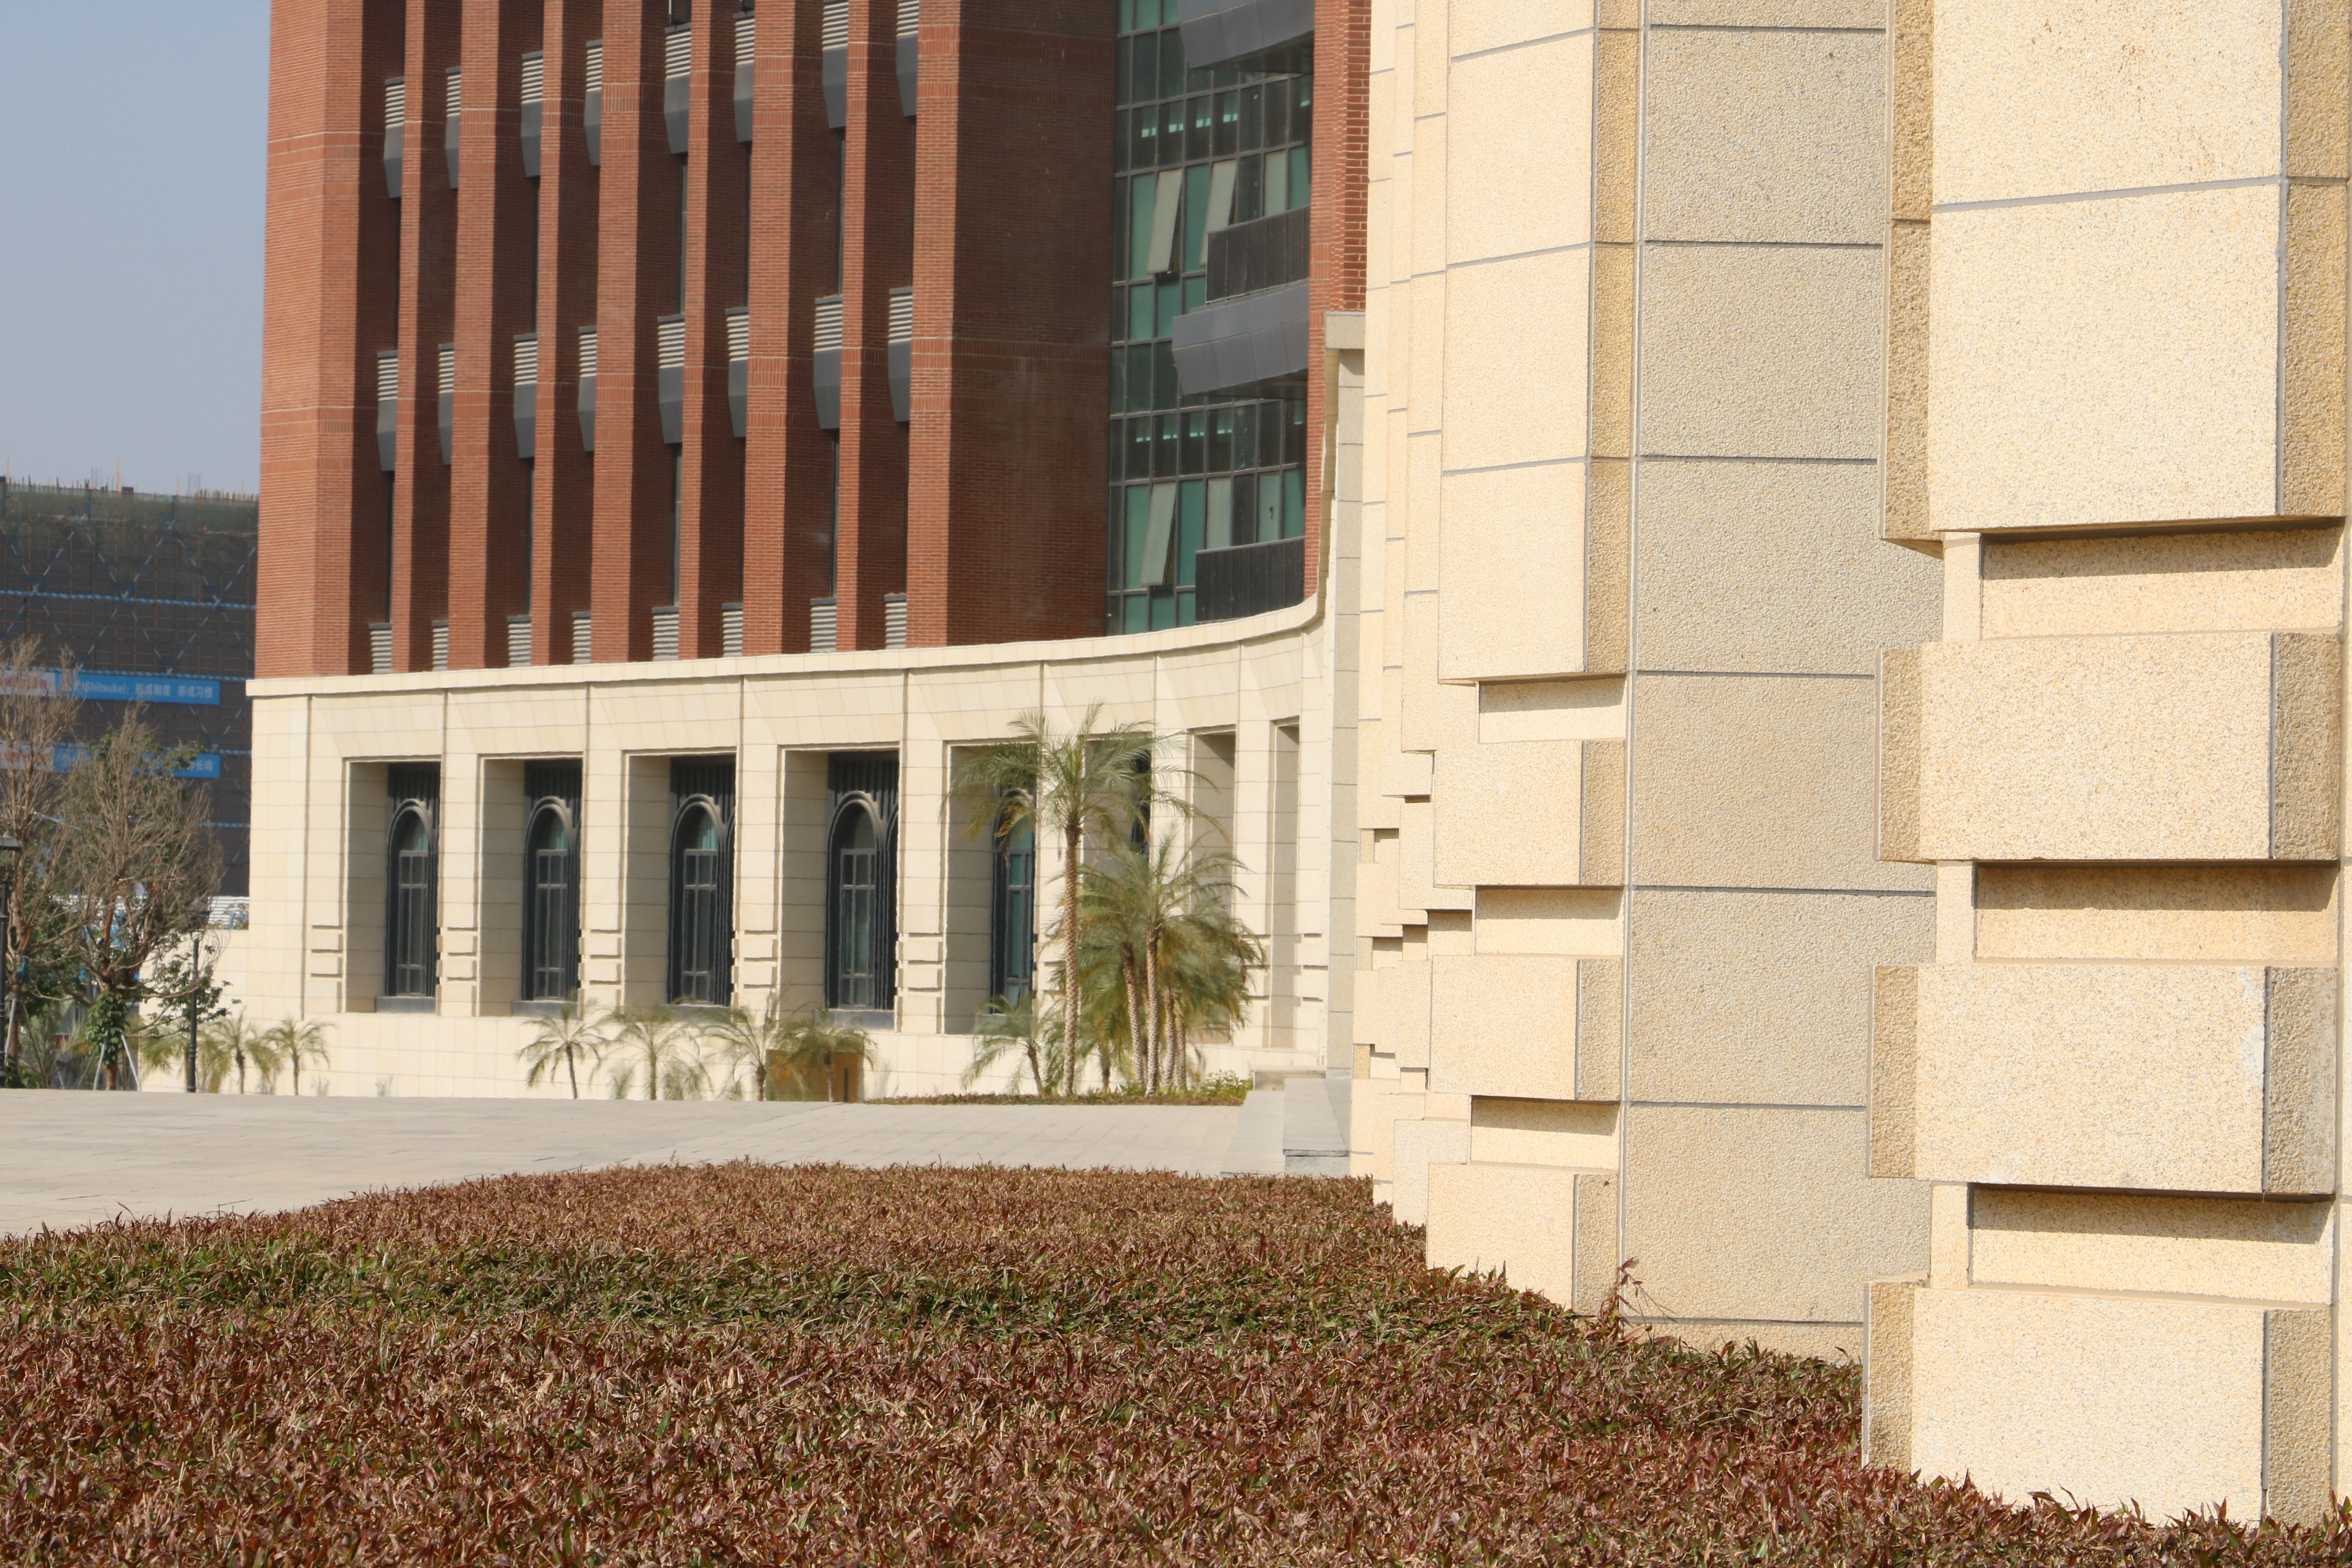
\includegraphics[width=1.0% 图片尺寸,可自行调节
		\textwidth]{images/1.jpg}% 图片名称(图片需与tex文件在同一文件夹)
		\caption{\fontsize{10pt}{15pt}\selectfont 校园风景}% 图例
        \label{fig:1}
	\end{minipage}
    \end{figure}

    \subsection{双图}
    \begin{figure}[H]% 插入两张图片并且并排
            
    	\centering
    	\begin{minipage}{0.48\textwidth}
    		\centering
    		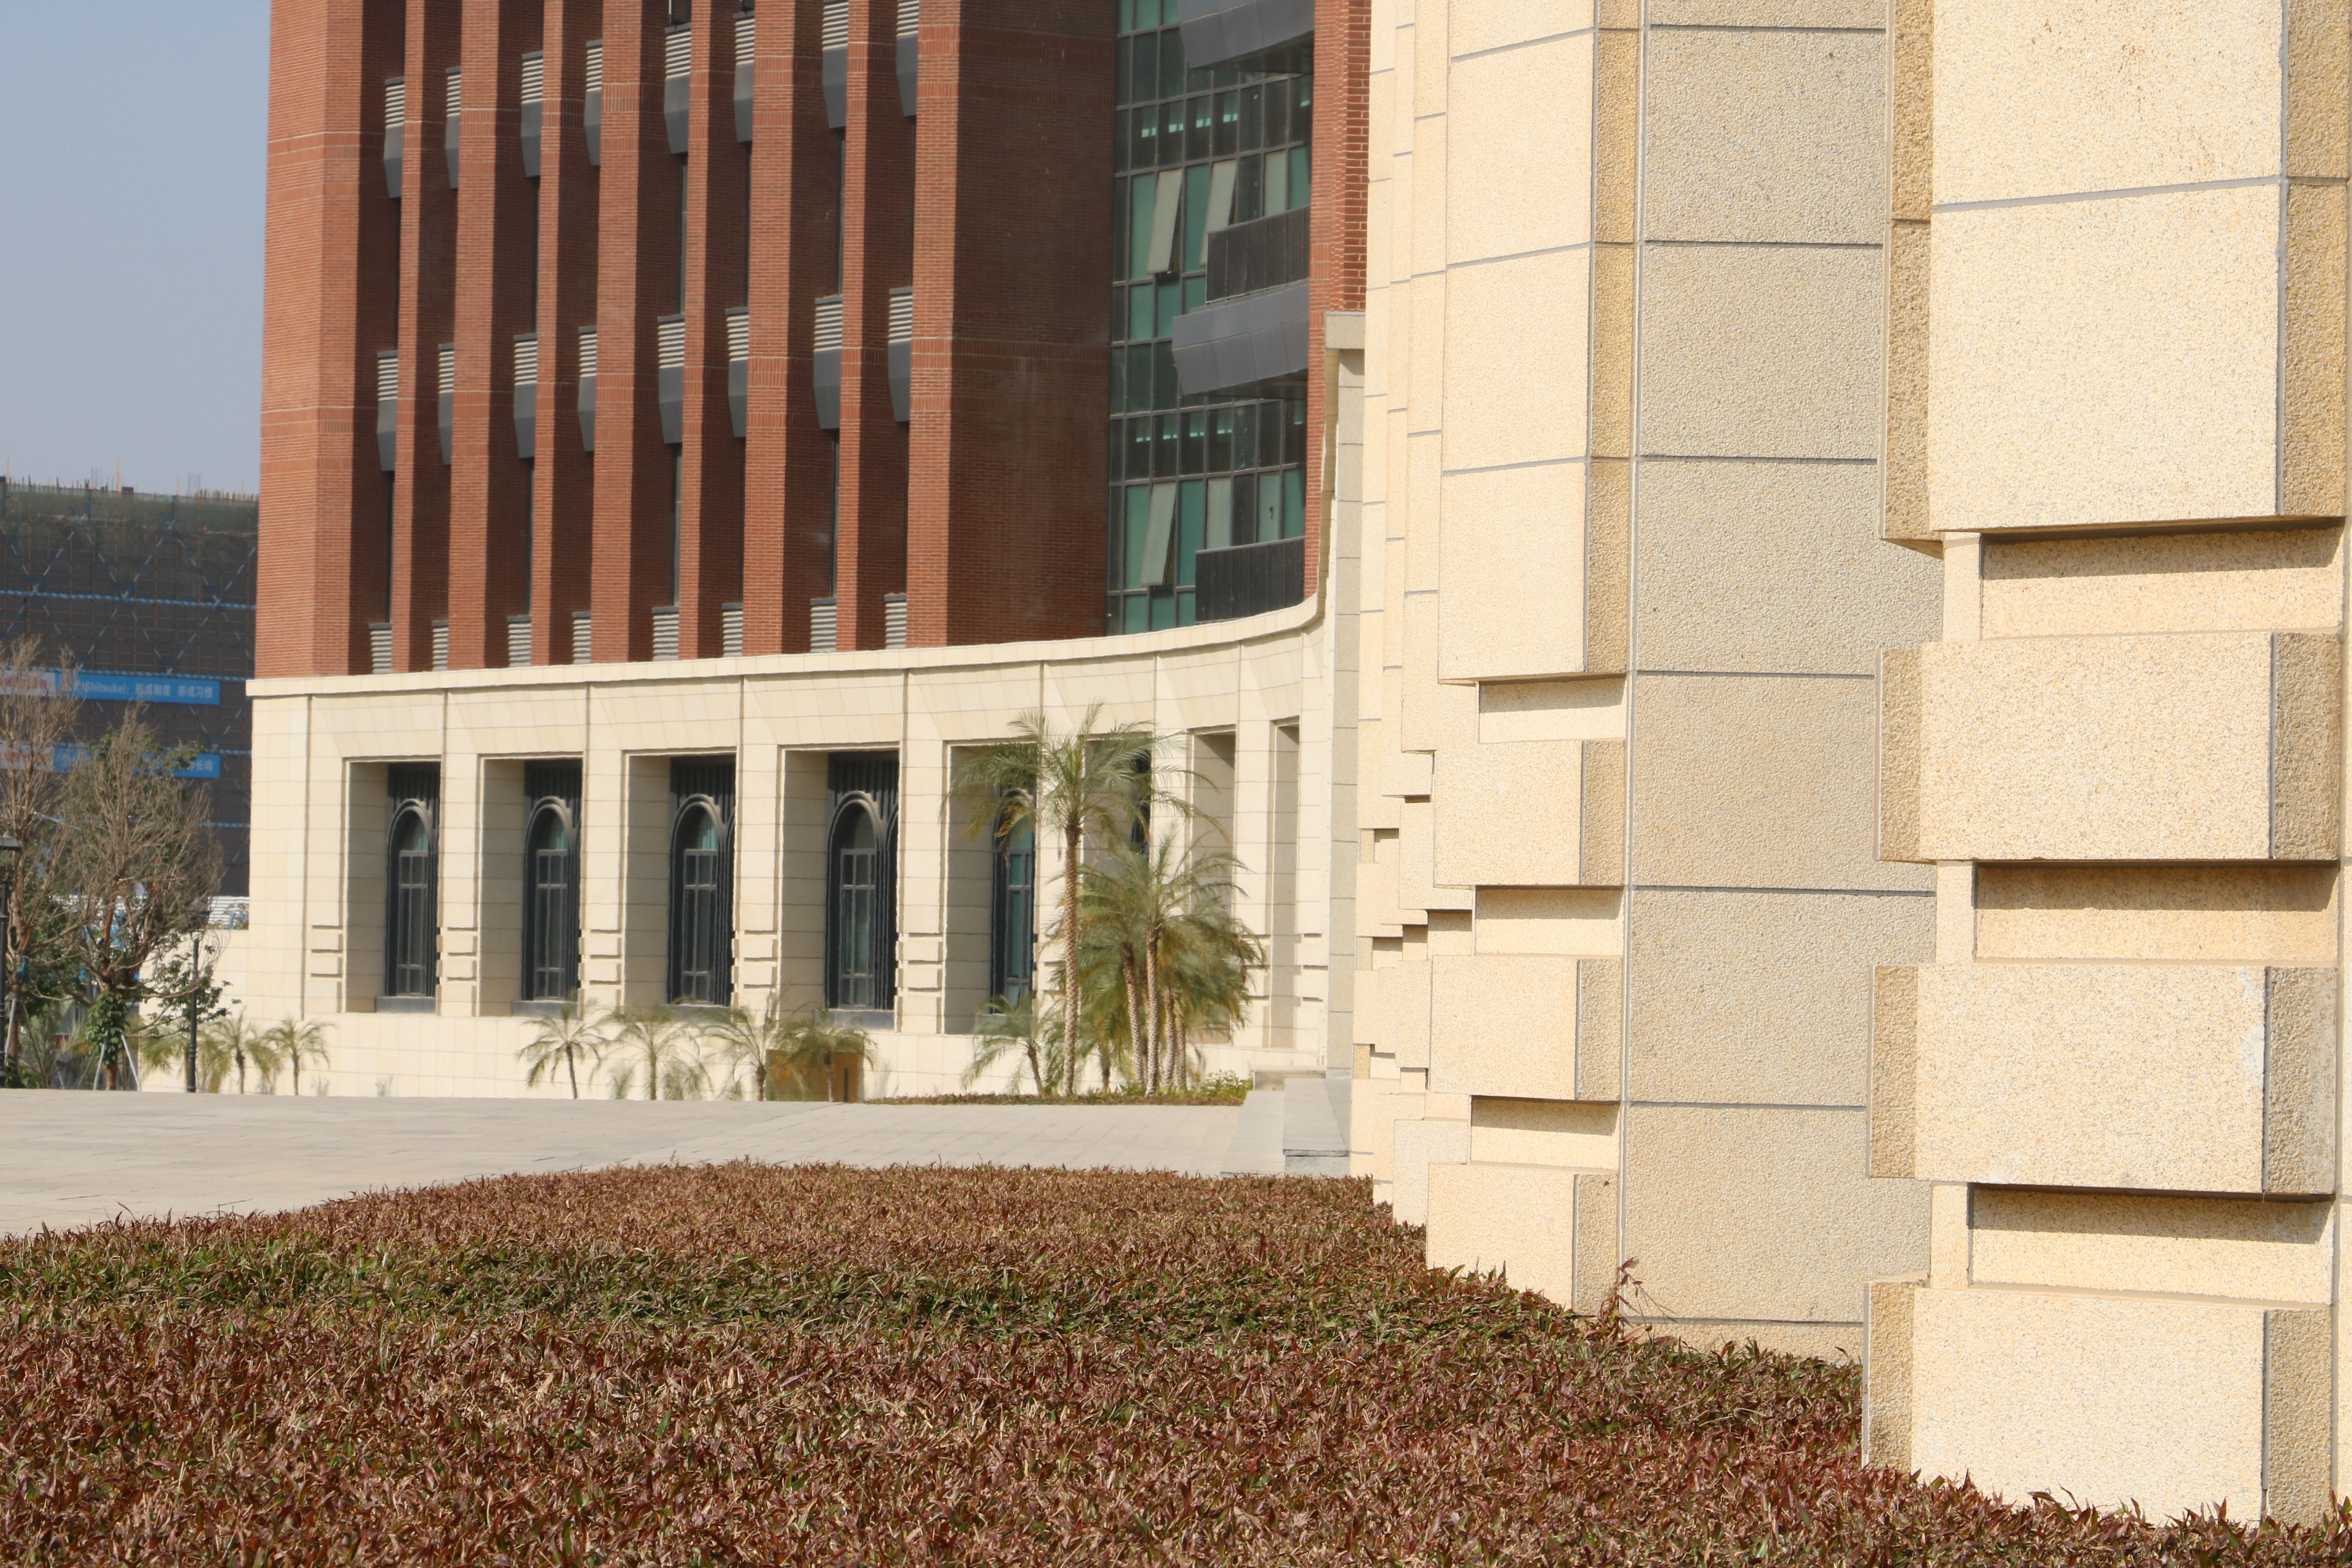
\includegraphics[width=0.83\textwidth]{images/1.jpg}
    		\caption{\fontsize{10pt}{15pt}\selectfont 校园风景}
    	\end{minipage}
    	\hspace{0cm}% 图片间距
    	\hfill% 撑满整行
    	\begin{minipage}{0.48\textwidth}
    		\centering
    		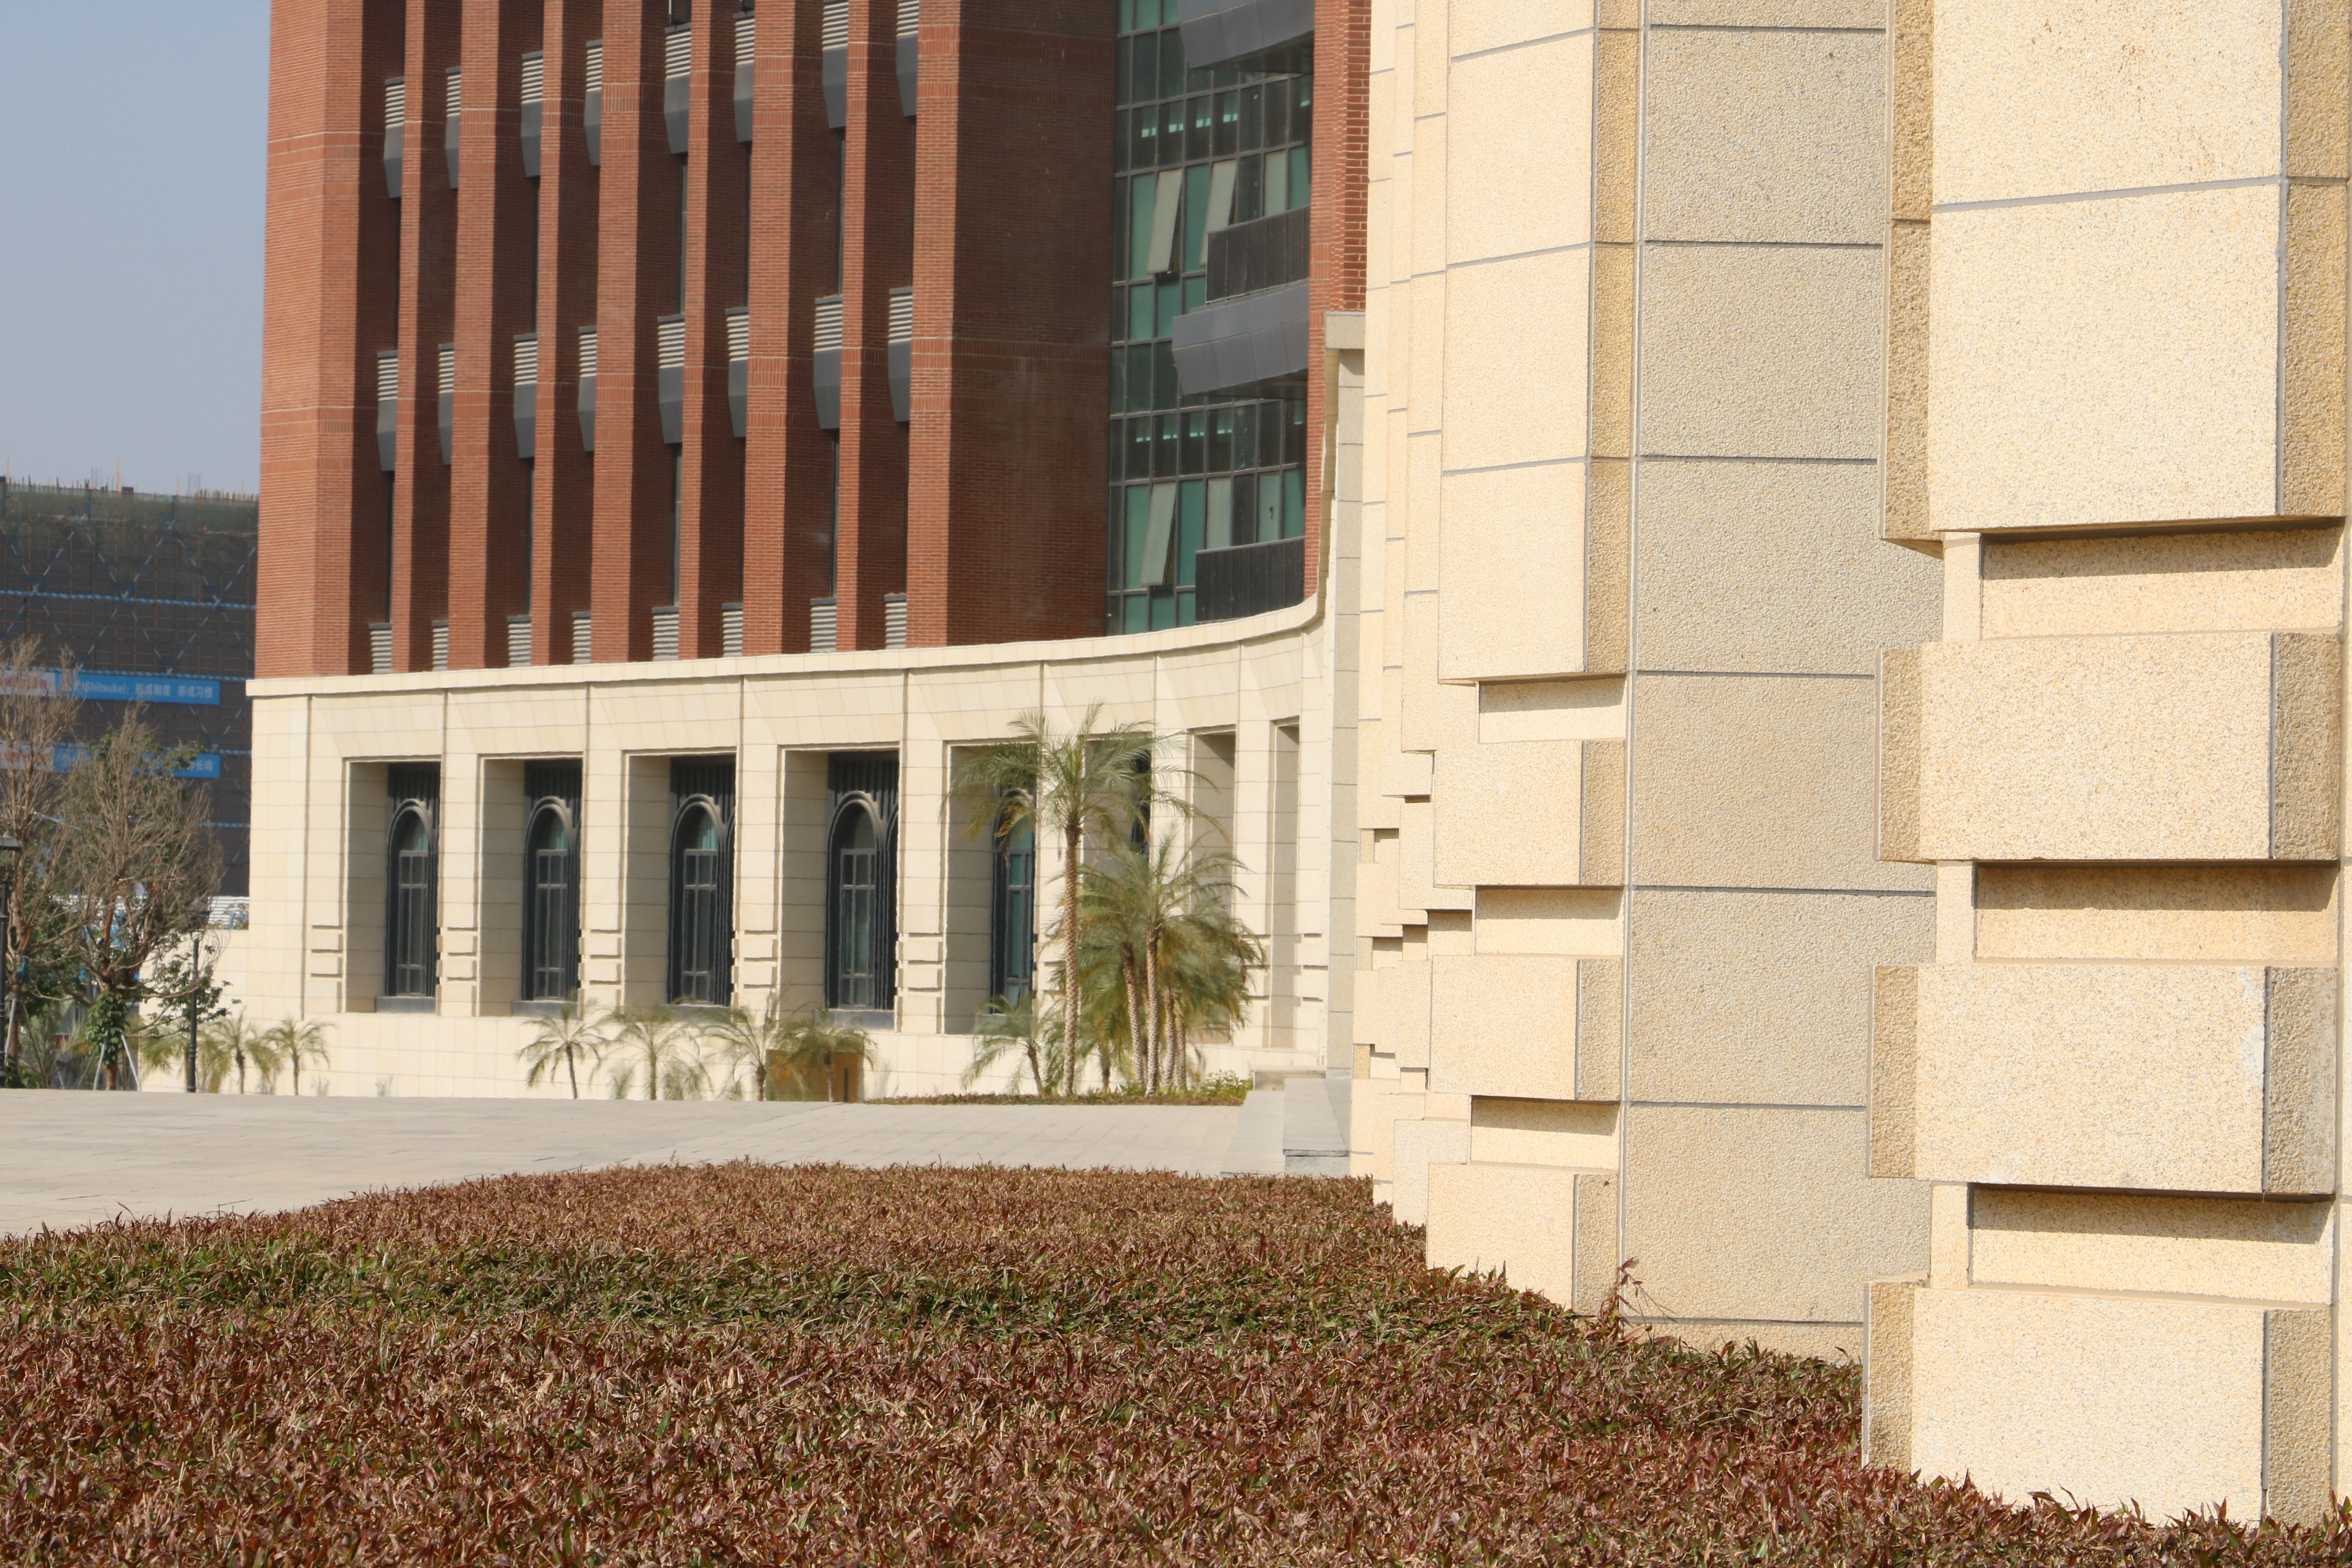
\includegraphics[width=0.83\textwidth]{images/1.jpg}
    		\caption{\fontsize{10pt}{15pt}\selectfont 校园风景}
    	\end{minipage}
    \end{figure}
    \subsection{四图}
    \begin{figure}[htbp]
        \centering
        \subfigure[校园风景]{
        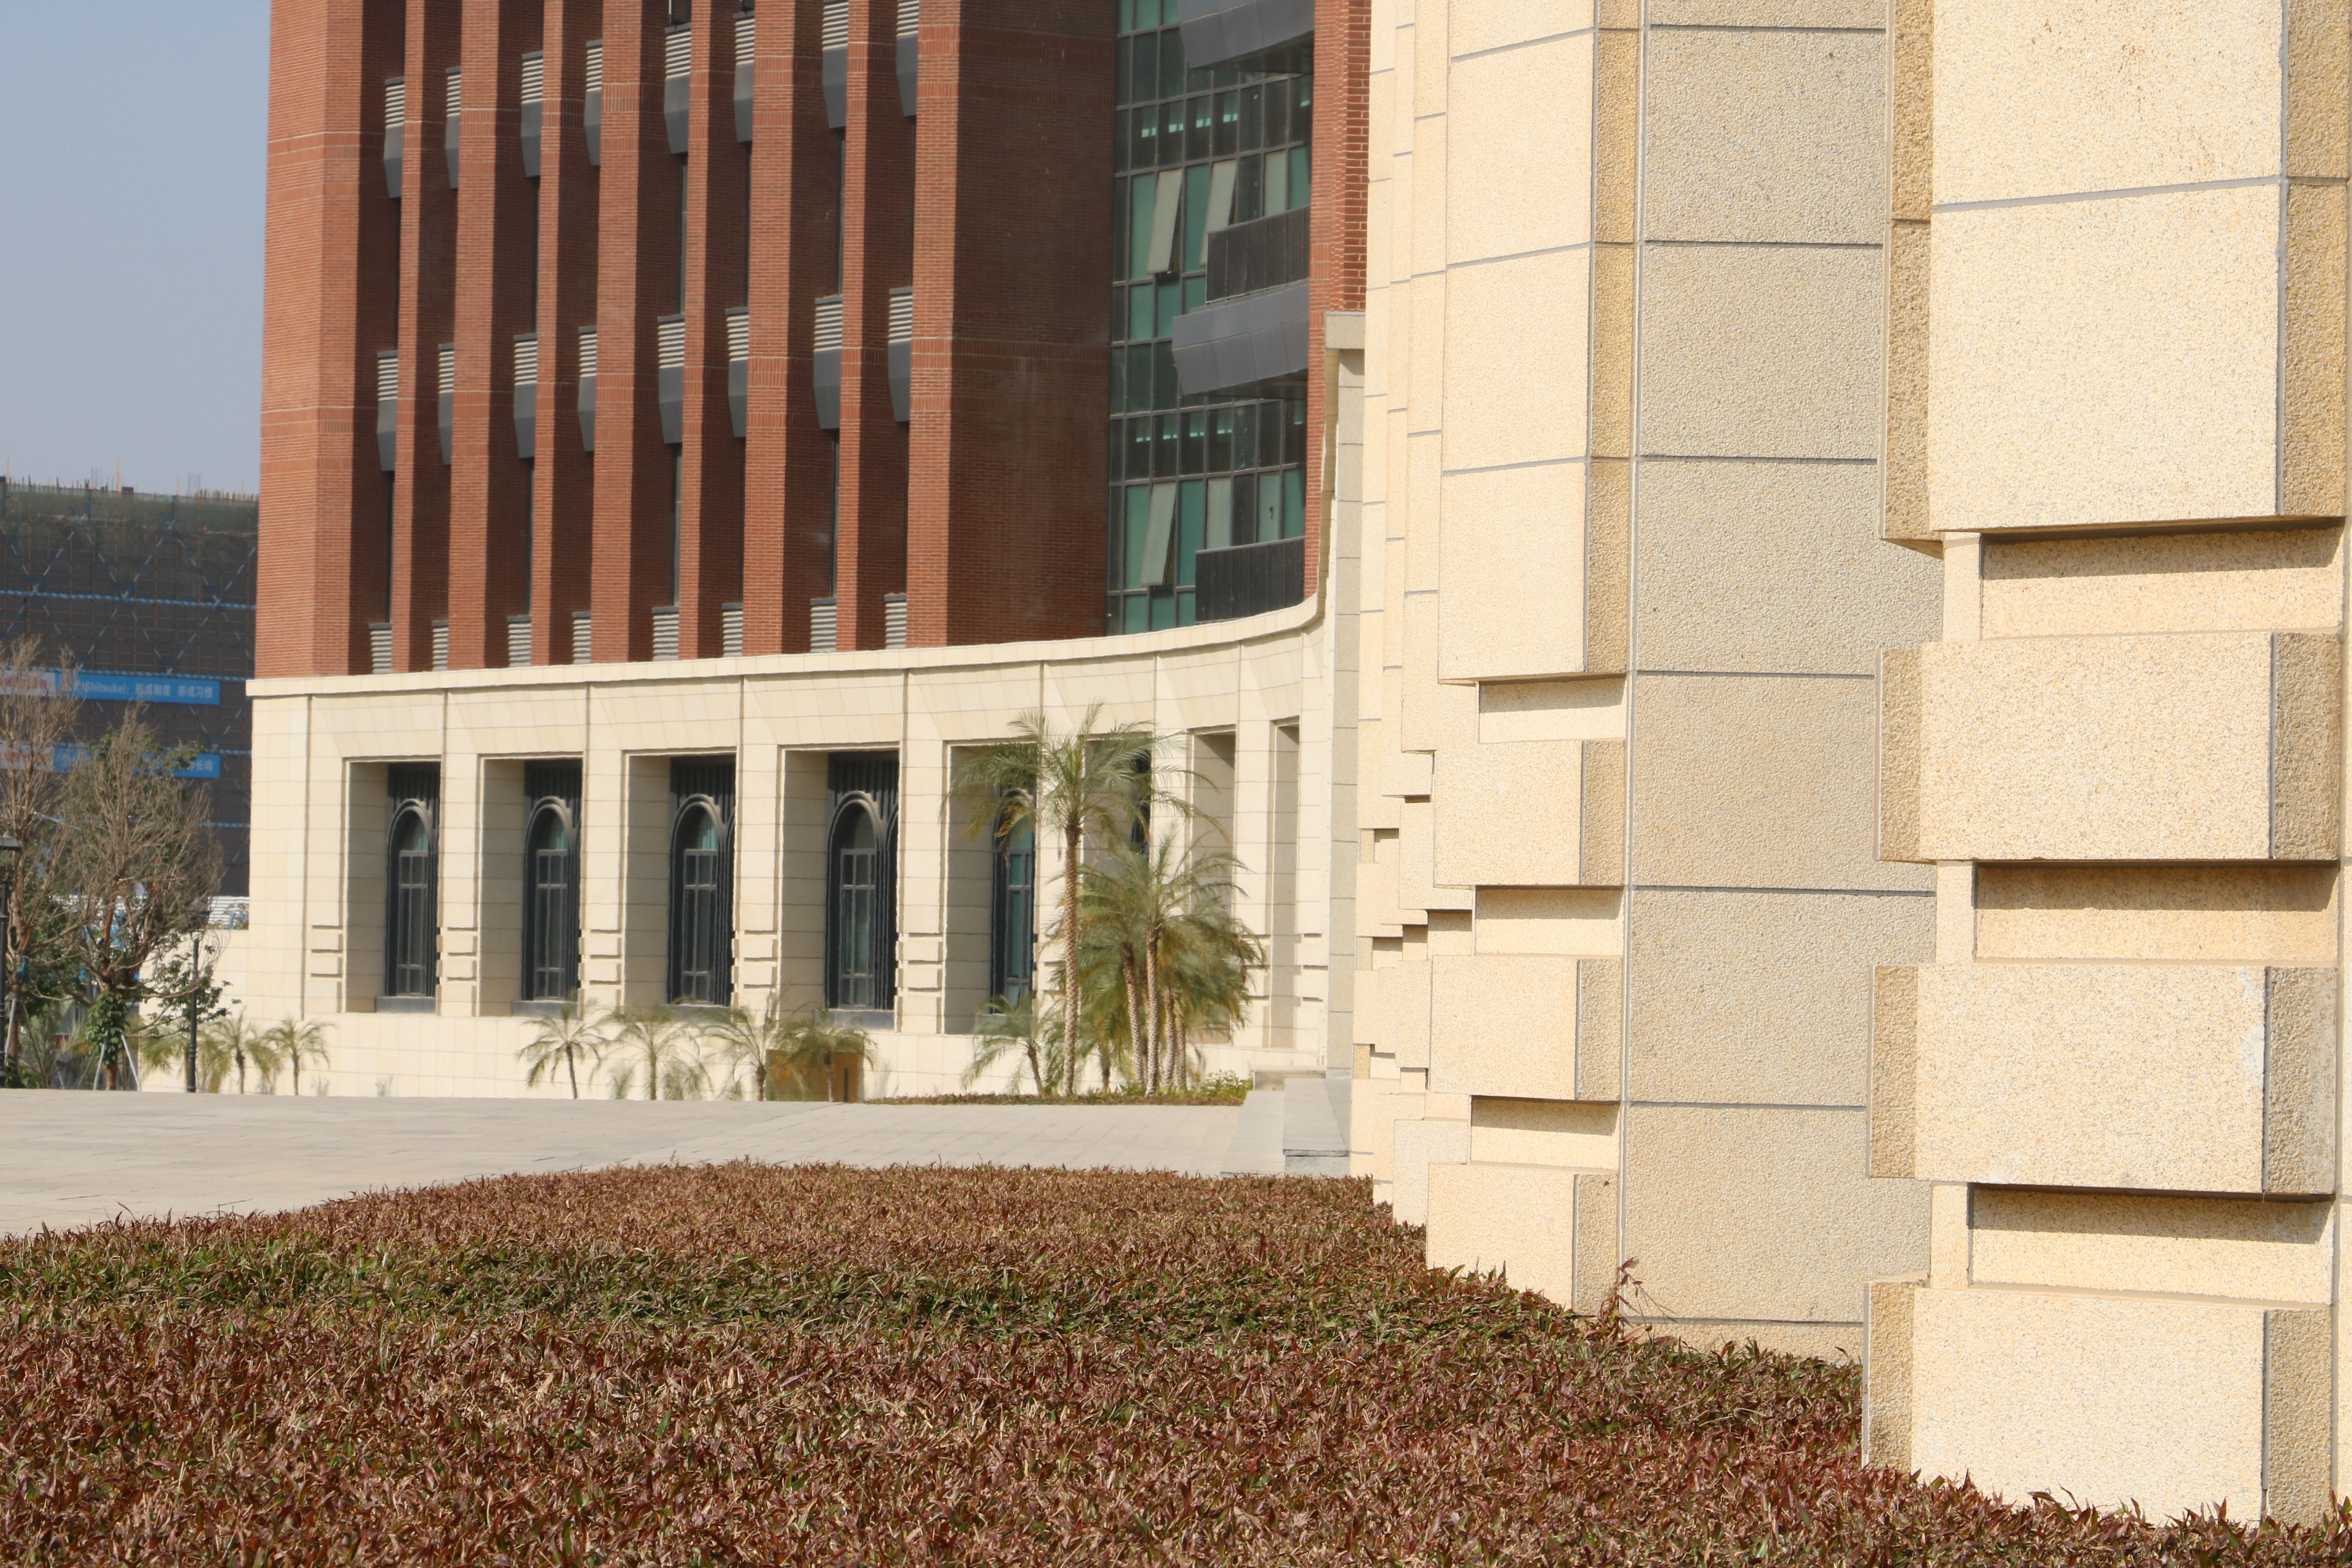
\includegraphics[width=5.5cm]{images/1.jpg}
        %\caption{fig1}
        }
        \quad
        \subfigure[校园风景]{
        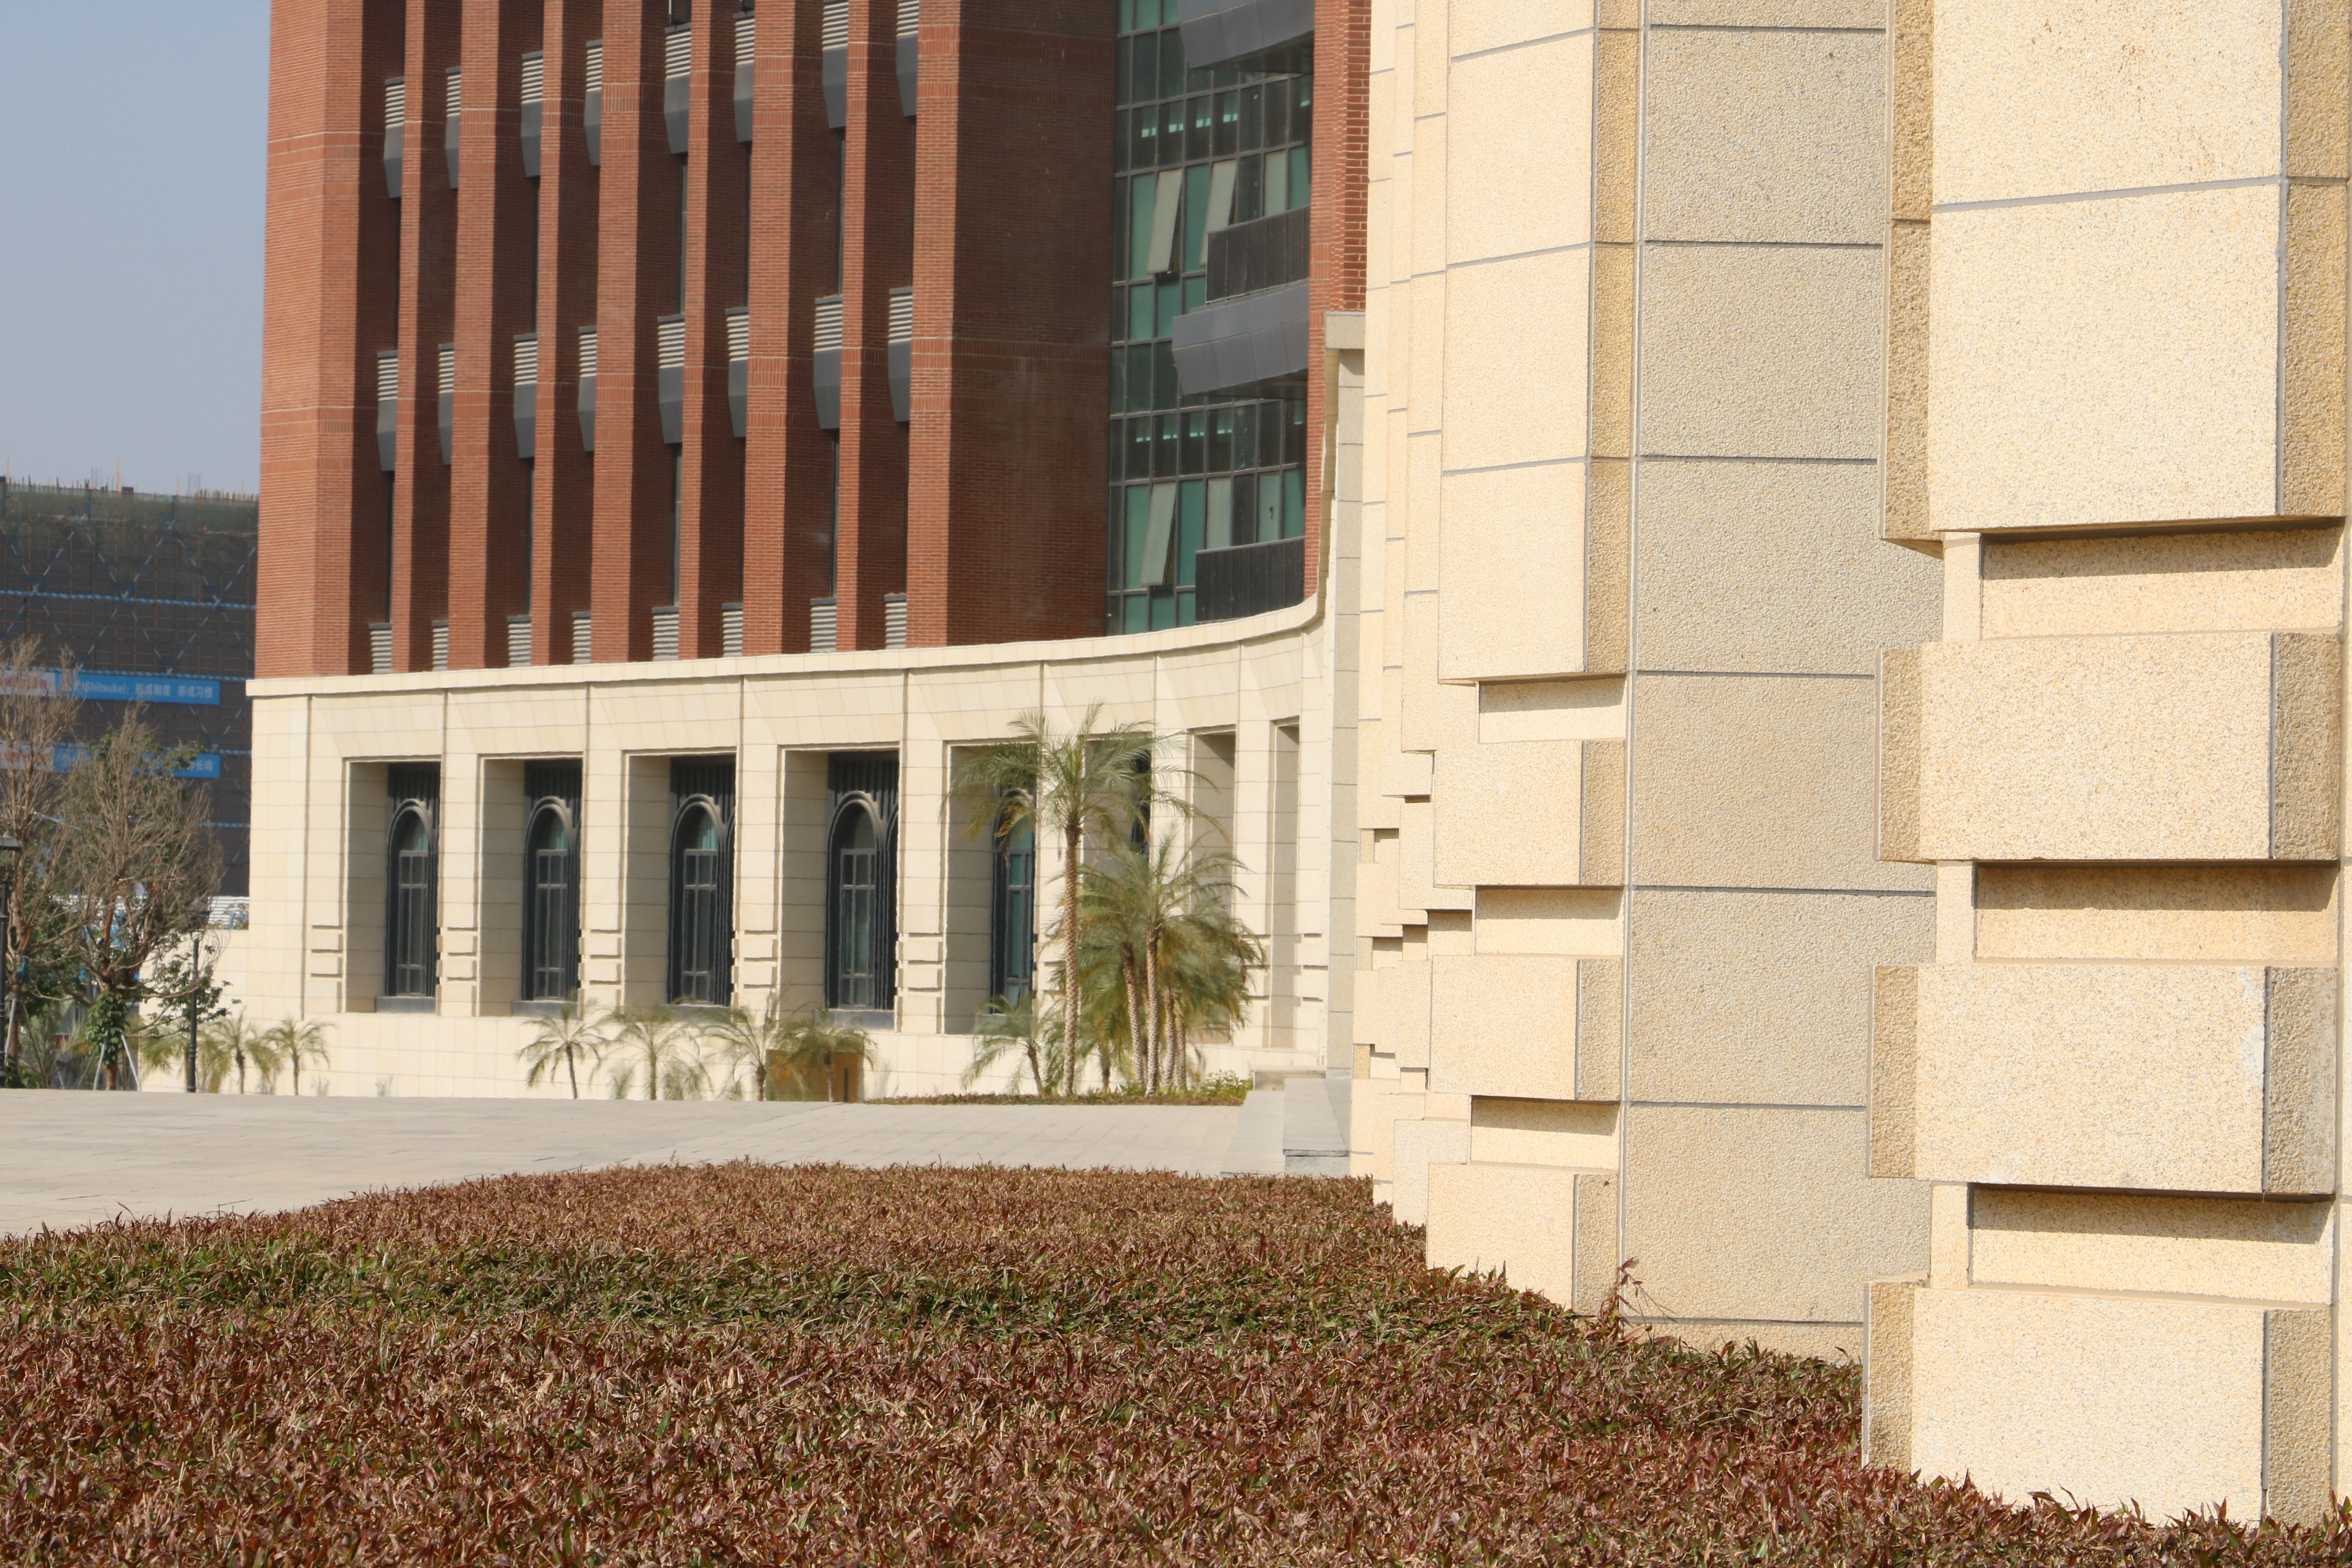
\includegraphics[width=5.5cm]{images/1.jpg}
        }
        \quad
        \subfigure[校园风景]{
        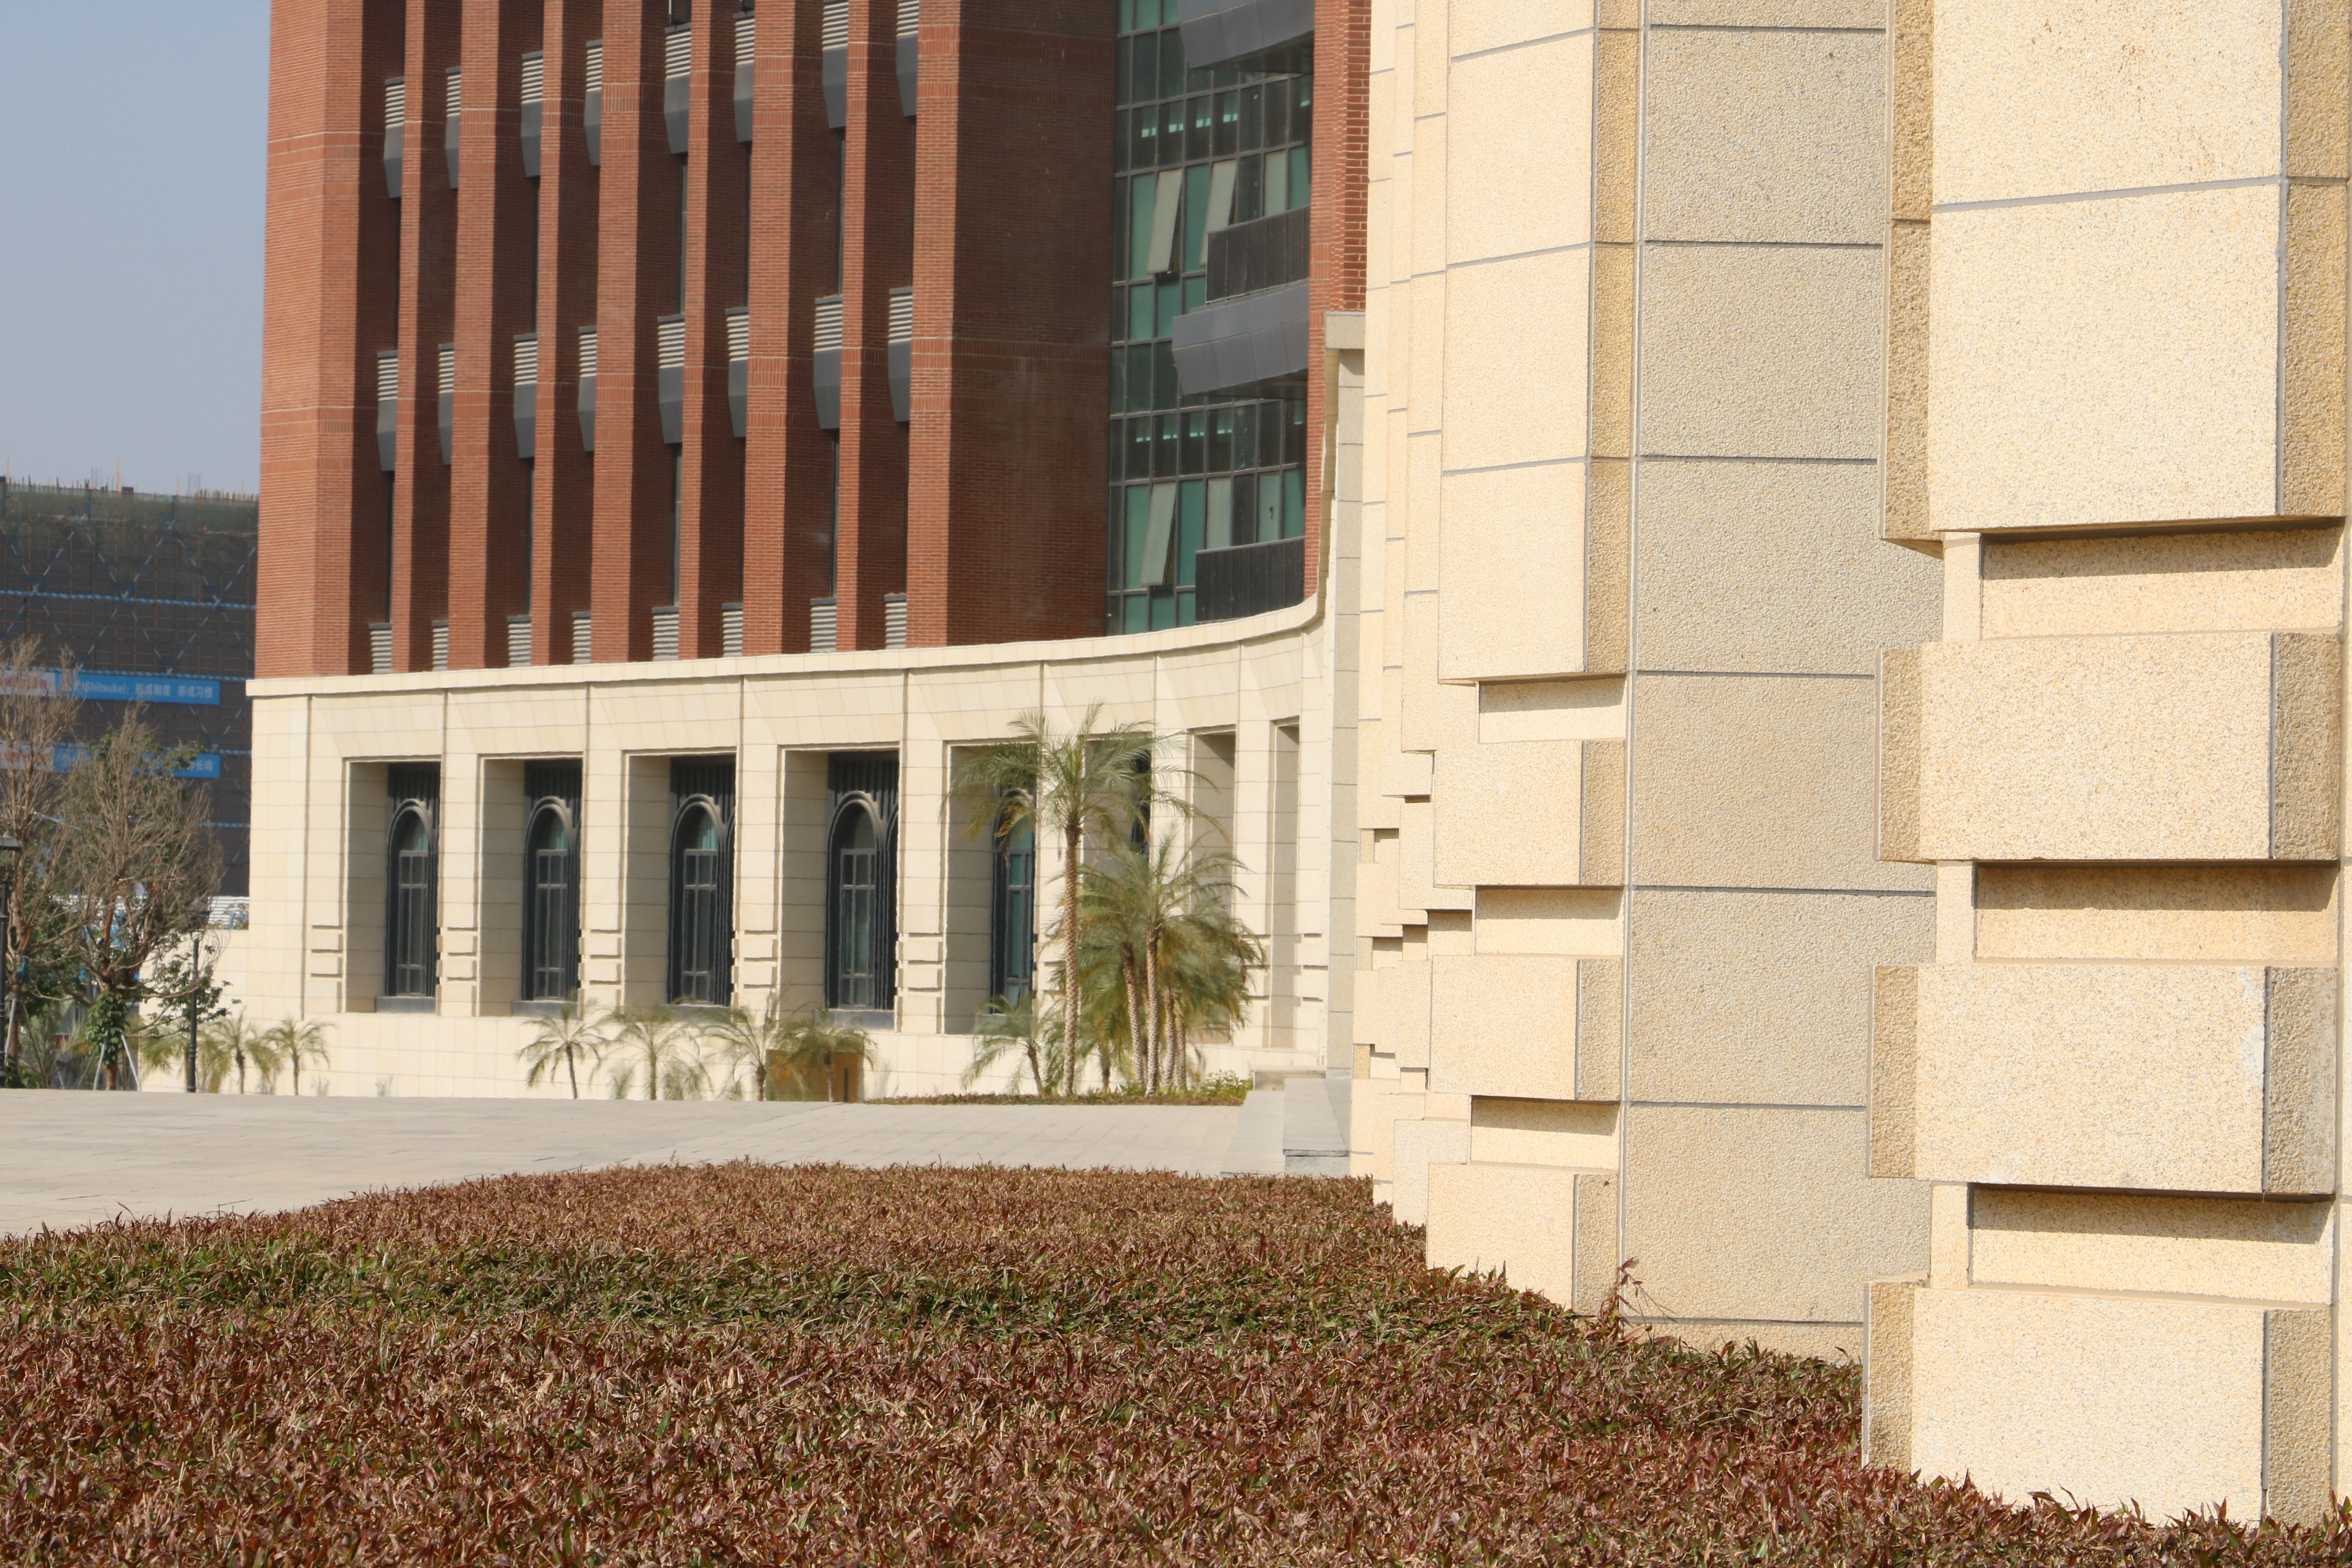
\includegraphics[width=5.5cm]{images/1.jpg}
        }
        \quad
        \subfigure[校园风景]{
        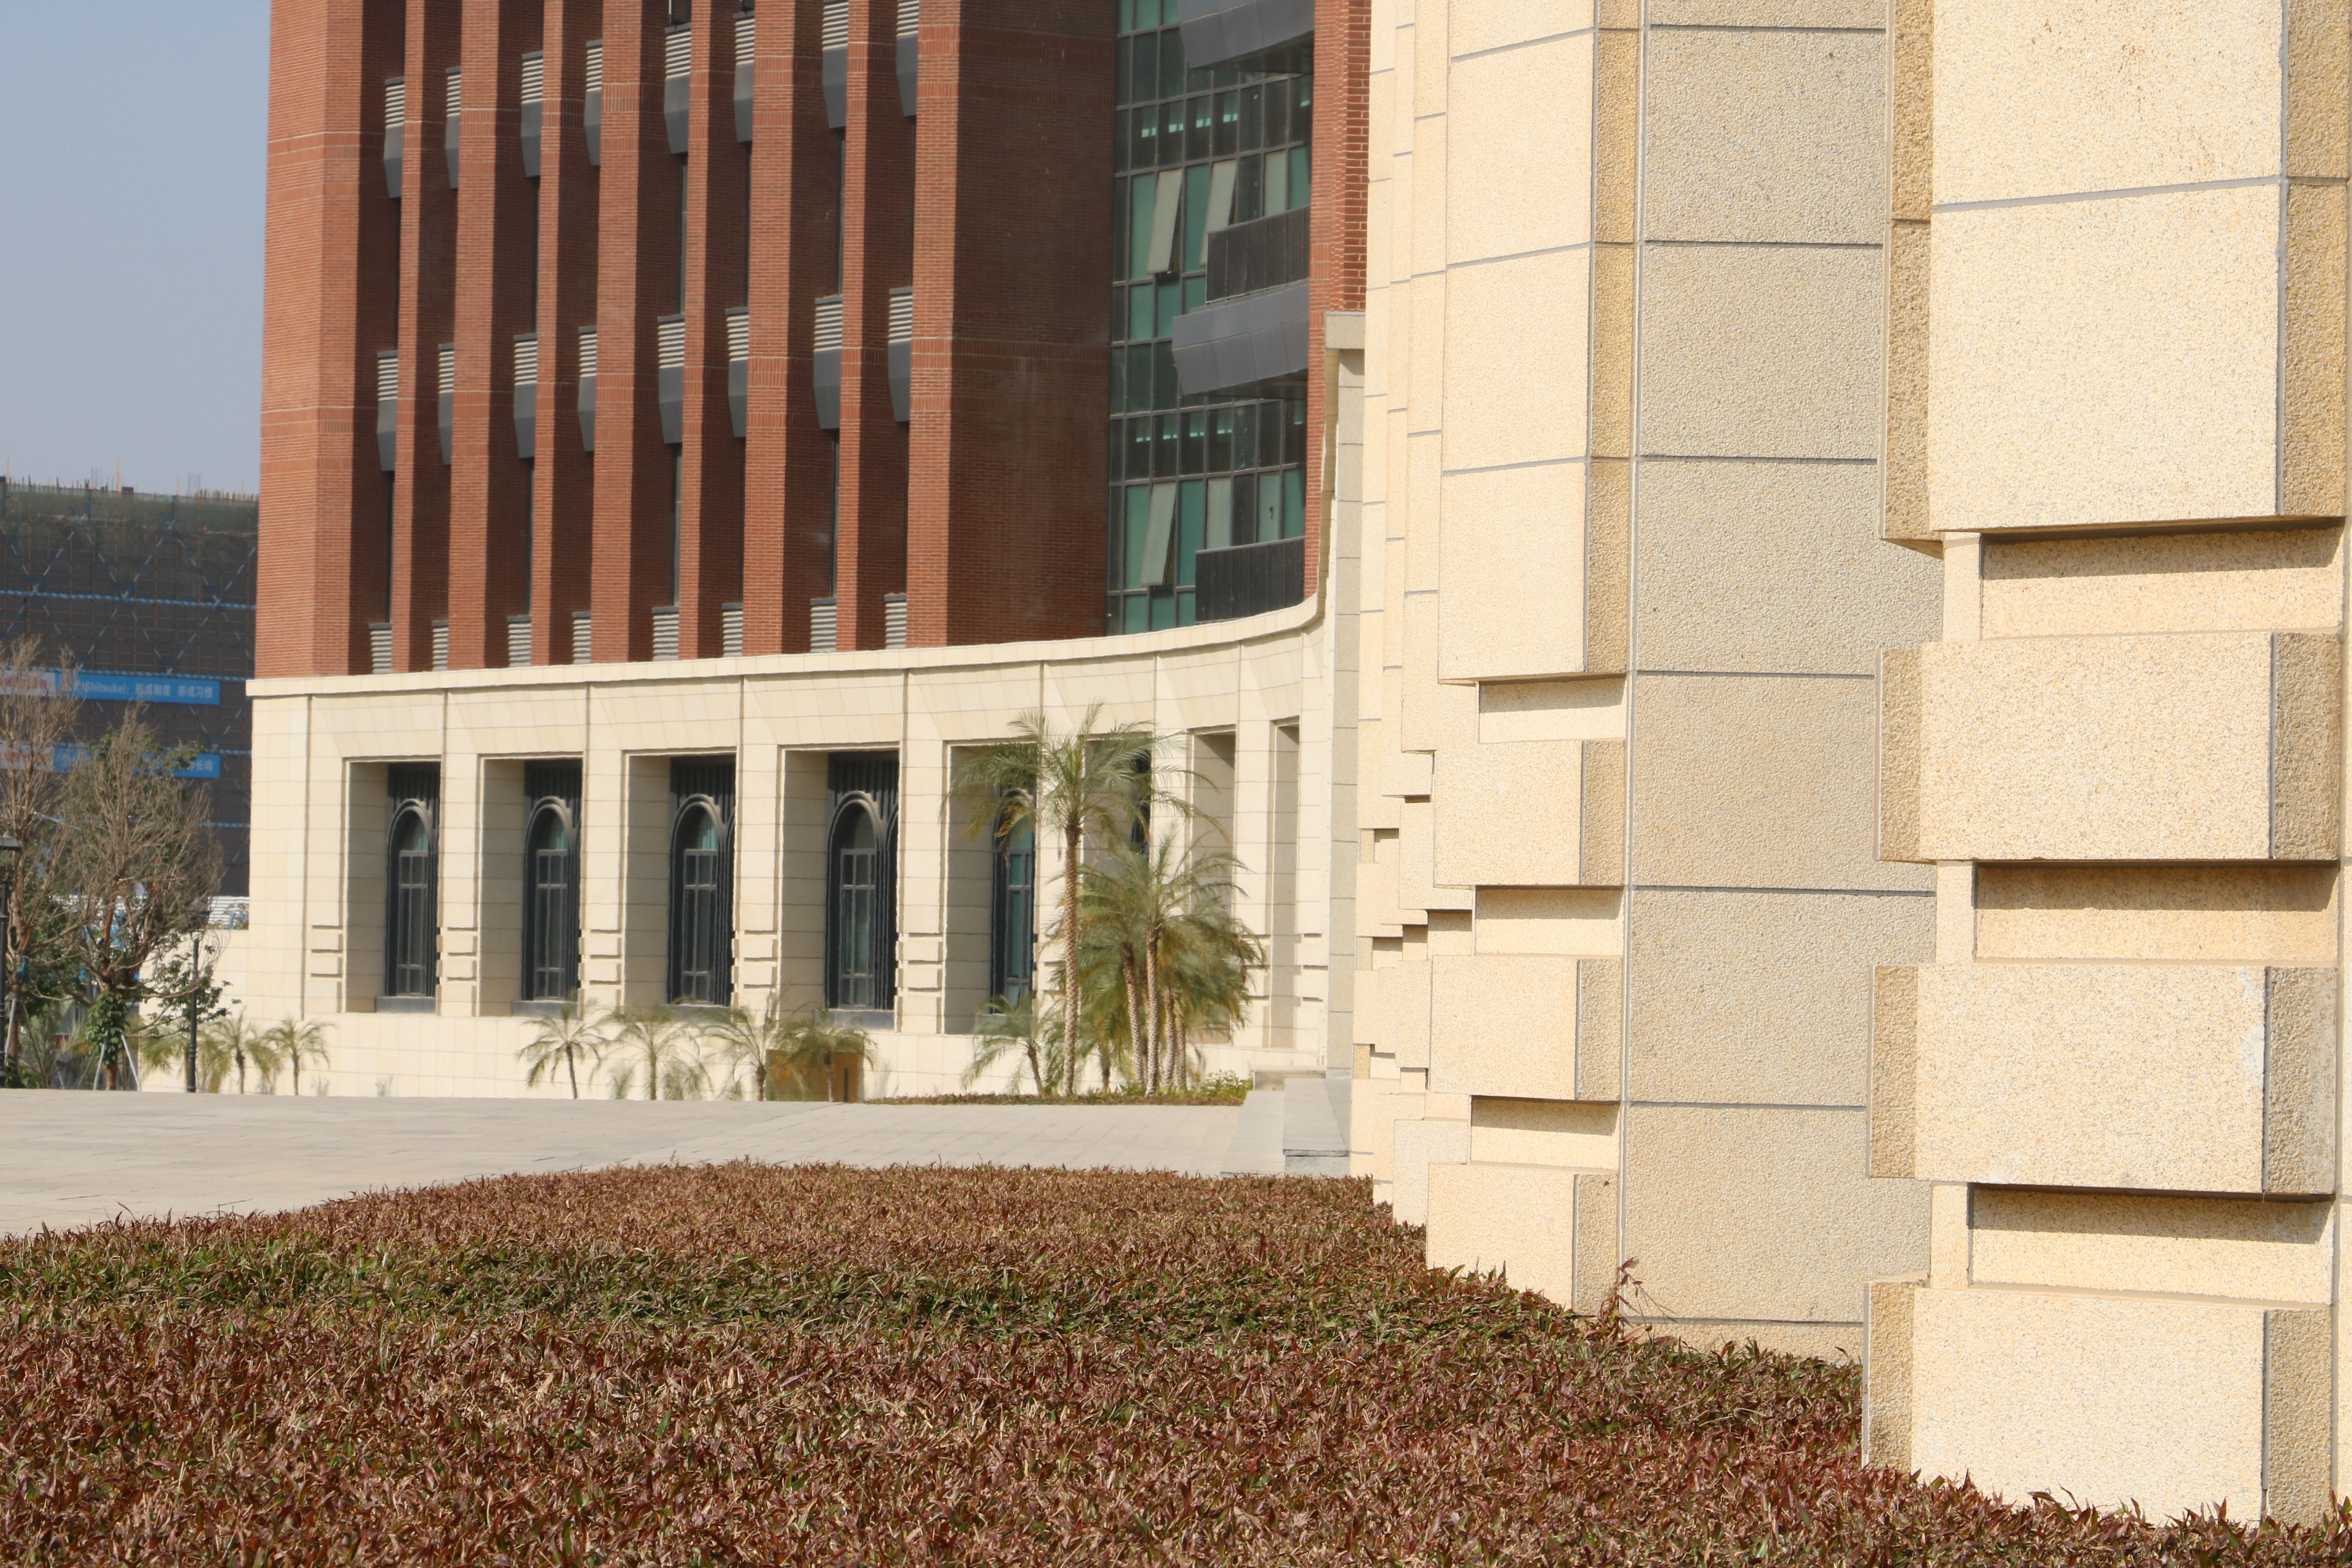
\includegraphics[width=5.5cm]{images/1.jpg}
        }
        \caption{ 校园风景}
    \end{figure}
    
    \section{插入表格}
    %%%%%%%%%%%%%%%%%%%%%%%%%%%%% 网站给表 %%%%%%%%%%%%%%%%%%%%%%%%%%%%
    \begin{table}[H]% 插入表格
    	\centering
            
    	\begin{tabular}{|l|l|l|l|l|}
    		\hline
    		$R_1$ & $R_2$ & $L$ & $V_1$ & $V_2$ \\ \hline
    		1mm & 1mm & 100mm & 2V & \makecell{表格内\\ 换行} \\ \hline
    	\end{tabular}
            \caption{\fontsize{10pt}{15pt}\selectfont 方块表}
            \label{table:1}
    \end{table}
    %%%%%%%%%%%%%%%%%%%%%%%%%%%%% 三线表 %%%%%%%%%%%%%%%%%%%%%%%%%%%%%%
    \begin{table}[H]% 插入表格
    	\centering
    	\caption{\fontsize{10pt}{15pt}\selectfont 三线表}
    	\begin{tabular}{ccccc}
        	\toprule[2pt]
    		$R_1$/mm & $R_2$/mm & $L$/mm & $V_1$/V & $V_2$/V \\ 
    	\midrule
    		2 & 1.5 & 190 & 6.55 & 0 \\ 
    	\bottomrule[2pt]
    	\end{tabular}
    \end{table}

    \section{插入公式}

    \subsection{单个公式}
    \begin{equation}% 单个公式
    	C_0=\frac{2V_1\text{arcth}\left[ \frac{\left( L+R_1-R_2 \right) \left( L-R_1-R_2 \right)}{\left( L+R_1+R_2 \right) \left( L-R_1+R_2 \right)} \right] ^{\frac{1}{2}}}{\text{arch}\left( \frac{L^2-R_{1}^{2}-R_{2}^{2}}{2R_1R_2} \right)}+\frac{2V_2\text{arcth}\left[ \frac{\left( L+R_2-R_1 \right) \left( L-R_1-R_2 \right)}{\left( L+R_1+R_2 \right) \left( L-R_2+R_1 \right)} \right] ^{\frac{1}{2}}}{\text{arch}\left( \frac{L^2-R_{1}^{2}-R_{2}^{2}}{2R_1R_2} \right)}
        \label{eq:1}
    \end{equation}
    
    \subsection{多行公式}
    \begin{equation}
    	\centering
    	\begin{split}% 多个公式
    		A_0&=\frac{V_2-V_1}{\ln \dfrac{R_{2}^{'}}{R_{1}^{'}}}\\
    		C_0&=\frac{V_1\ln R_{2}^{'}-V_2\ln R_{1}^{'}}{\ln \dfrac{R_{2}^{'}}{R_{1}^{'}}}
    	\end{split}
    \end{equation}

    \subsection{对齐公式}
    \begin{align}% 对齐公式
    		A_0&=3c+6666\\% 注意换行
    		&=369
    \end{align}

    \section{引用格式}
    图片引用格式:如图\ref{fig:1}所示,注意引用时最好\textcolor{blue}{$\backslash$label}放在\textcolor{blue}{$\backslash$caption}后面,避免有些情况会报错。

    表格引用格式:如表\ref{table:1}所示。

    公式引用格式:如式\eqref{eq:1}所示。

    文献引用通过\textcolor{blue}{$\backslash$bibliography}实现,在文件main.bib中加入BibTeX格式的参考文献信息,如编码缓存\cite{maddah2014fundamental}。
    


    \bibliographystyle{gbt7714-numerical}
    \bibliography{main}
\end{document}% 结束文档编辑,后面写啥都编译不出来